\documentclass[11pt,a4paper]{article}
\usepackage[utf8]{inputenc}
\usepackage[vietnamese]{babel}
\usepackage{amsmath,amssymb}
\usepackage[version=4]{mhchem}
\usepackage{geometry}
\geometry{top=1.5cm,bottom=1.2cm,left=1.4cm,right=1.4cm,headheight=28pt,headsep=12pt,footskip=18pt}
\usepackage{graphicx}
\usepackage{xcolor}
\usepackage{tabularx}
\usepackage{array}
\usepackage{tikz}
\usepackage{fancyhdr}
\usepackage{enumitem}
\usepackage{multido}
\usepackage{tcolorbox}
\usepackage{colortbl}

\definecolor{hfRed}{HTML}{D32F2F}
\definecolor{hfGreen}{HTML}{8BC390}
\definecolor{mainGreen}{HTML}{2E7D32}
\definecolor{solBlue}{HTML}{1565C0}
\definecolor{tableGreen}{HTML}{E8F5E9}

\usepackage{ex_test}

\pagestyle{fancy}
\fancyhf{}
\renewcommand{\headrulewidth}{0.75pt}
\renewcommand{\headrule}{\hbox to\headwidth{\color{hfGreen}\leaders\hrule height \headrulewidth\hfill}}
\renewcommand{\footrulewidth}{0.75pt}
\renewcommand{\footrule}{\hbox to\headwidth{\color{hfGreen}\leaders\hrule height \footrulewidth\hfill}}

\fancyhead[L]{\small\itshape\color{hfRed}Tài liệu lưu hành nội bộ}
\fancyhead[R]{\small\color{hfRed}Thầy \textbf{TRẦN VĂN THẠNH} - 0777.470.803}

\fancyfoot[L]{\footnotesize\itshape\color{hfRed}CS1: 6/15 Nguyễn Hoàng, P. Kim Long, TP Huế \quad|\quad CS2: 24 Đặng Thái Thân, TP Huế}
\fancyfoot[R]{\small\textbf{\color{hfRed}Trang \thepage}}

\setlength{\parindent}{0pt}
\setlength{\parskip}{2pt}

\begin{document}

\begin{minipage}[t]{0.48\textwidth}
\textbf{TRƯỜNG THPT NGUYỄN HUỆ}\\
\textbf{TỔ LÝ – HOÁ – CN}\\
\textit{ĐỀ CHÍNH THỨC}\\
\textit{(Đề thi có 04 trang)}
\end{minipage}
\hfill
\begin{minipage}[t]{0.48\textwidth}
\raggedleft
\textbf{\color{hfRed}KIỂM TRA GIỮA KỲ I – NĂM HỌC 2026 – 2027}\\
\textbf{Môn: HOÁ HỌC, Lớp 11}\\
\textit{Thời gian: 45 phút (không kể thời gian phát đề)}\\
\textbf{MÃ ĐỀ: 1204}
\end{minipage}

\vspace{4pt}
\noindent
\textit{Họ và tên thí sinh:} \dotfill \textit{Lớp:} \dotfill \textit{SBD:} \dotfill

\vspace{2pt}
\noindent
\textit{\footnotesize (Cho biết nguyên tử khối: $\ce{H = 1; N = 14; O = 16; K = 39; Ca = 40}$).}

\vspace{2pt}
\hrule color{hfGreen} height 0.5pt


\vspace{4pt}
\begin{center}
\textbf{\color{hfRed}\large (BẢN GIÁO VIÊN -- CÓ LỜI GIẢI CHI TIẾT)}
\end{center}

\vspace{2pt}
\begin{center}
{\color{hfRed}\textbf{\large BẢNG ĐÁP ÁN RÚT GỌN (DÀNH CHO GIÁO VIÊN)}}
\end{center}

\vspace{2pt}
\noindent
\textbf{\color{mainGreen}1. Phần I: Trắc nghiệm nhiều lựa chọn (3,0 điểm - mỗi câu đúng 0,25 điểm)}
\begin{center}
\renewcommand{\arraystretch}{1.2}
\begin{tabular}{|c|c|c|c|c|c|c|c|c|c|c|c|c|}
\hline
\rowcolor{tableGreen}
\textbf{Câu} & \textbf{1} & \textbf{2} & \textbf{3} & \textbf{4} & \textbf{5} & \textbf{6} & \textbf{7} & \textbf{8} & \textbf{9} & \textbf{10} & \textbf{11} & \textbf{12} \\
\hline
\textbf{Đ/A} & \textbf{\color{hfRed}B} & \textbf{\color{hfRed}C} & \textbf{\color{hfRed}D} & \textbf{\color{hfRed}B} & \textbf{\color{hfRed}A} & \textbf{\color{hfRed}B} & \textbf{\color{hfRed}C} & \textbf{\color{hfRed}A} & \textbf{\color{hfRed}B} & \textbf{\color{hfRed}A} & \textbf{\color{hfRed}B} & \textbf{\color{hfRed}B} \\
\hline
\end{tabular}
\end{center}

\vspace{2pt}
\noindent
\textbf{\color{mainGreen}2. Phần II: Trắc nghiệm Đúng / Sai (2,0 điểm)}
\begin{center}
\renewcommand{\arraystretch}{1.2}
\begin{tabular}{|c|c|c|c|c|}
\hline
\rowcolor{tableGreen}
\textbf{Câu} & \textbf{Lệnh a)} & \textbf{Lệnh b)} & \textbf{Lệnh c)} & \textbf{Lệnh d)} \\
\hline
\textbf{Câu 1} & \textbf{\color{hfRed}ĐÚNG} & \textbf{\color{solBlue}SAI} & \textbf{\color{solBlue}SAI} & \textbf{\color{hfRed}ĐÚNG} \\
\hline
\textbf{Câu 2} & \textbf{\color{hfRed}ĐÚNG} & \textbf{\color{hfRed}ĐÚNG} & \textbf{\color{solBlue}SAI} & \textbf{\color{solBlue}SAI} \\
\hline
\end{tabular}
\end{center}

\vspace{2pt}
\noindent
\textbf{\color{mainGreen}3. Phần III: Trắc nghiệm Trả lời ngắn (2,0 điểm - mỗi câu đúng 0,5 điểm)}
\begin{center}
\renewcommand{\arraystretch}{1.2}
\begin{tabular}{|c|c|c|c|c|}
\hline
\rowcolor{tableGreen}
\textbf{Câu hỏi} & \textbf{Câu 1} & \textbf{Câu 2} & \textbf{Câu 3} & \textbf{Câu 4} \\
\hline
\textbf{Đáp án} & \textbf{\color{hfRed}3} & \textbf{\color{hfRed}124} & \textbf{\color{hfRed}51,5} & \textbf{\color{hfRed}4312} \\
\hline
\end{tabular}
\end{center}

\vspace{4pt}
\hrule color{hfGreen} height 0.5pt


\vspace{4pt}
\noindent
\textbf{\large\color{hfRed}A. PHẦN TRẮC NGHIỆM (7,0 ĐIỂM)}

\vspace{2pt}
\noindent
\textbf{\large\color{mainGreen}PHẦN I. Câu trắc nghiệm nhiều phương án lựa chọn (3,0 điểm)}

\textit{Học sinh trả lời từ câu 1 đến câu 12. Mỗi câu hỏi học sinh chỉ chọn một phương án.}
\vspace{4pt}


\begin{ex}%[1204-C1]
Mưa acid là hiện tượng nước mưa có pH thấp hơn 5,6. Hai acid chủ yếu được hình thành trong khí quyển và hòa tan vào nước mưa, gây ra mưa acid là
\choice
{\ce{HCl}, \ce{HNO3}}
{\True \ce{H2SO4}, \ce{HNO3}}
{\ce{SO2}, \ce{NO_x}}
{\ce{H2SO4}, \ce{H2S}}
\begin{loigiai}
Khí $\ce{SO2}$ và các oxide của nitrogen ($\ce{NO_x}$) trong khí quyển bị oxi hóa bởi oxygen và hòa tan trong nước mưa tạo thành hai acid chủ yếu gây ra hiện tượng mưa acid là $\ce{H2SO4}$ và $\ce{HNO3}$.\\
$\rightarrow$ \textbf{Chọn đáp án B.}
\end{loigiai}
\end{ex}


\begin{ex}%[1204-C2]
Cho phương trình: $\ce{CO3^{2-} + H2O <=> HCO3^- + OH^-}$\\
Trong phản ứng thuận, theo thuyết Brønsted -- Lowry chất nào là base?
\choice
{\ce{HCO3^-}}
{\ce{OH^-}}
{\True \ce{CO3^{2-}}}
{\ce{H2O}}
\begin{loigiai}
Theo thuyết Brønsted -- Lowry, base là chất nhận proton ($\ce{H+}$). Trong phản ứng thuận:
$\ce{CO3^{2-} + H2O <=> HCO3^- + OH^-}$, ion $\ce{CO3^{2-}}$ nhận $\ce{H+}$ từ $\ce{H2O}$ để tạo thành $\ce{HCO3^-}$, do đó $\ce{CO3^{2-}}$ đóng vai trò là base (còn $\ce{H2O}$ nhường $\ce{H+}$ nên là acid).\\
$\rightarrow$ \textbf{Chọn đáp án C.}
\end{loigiai}
\end{ex}


\begin{ex}%[1204-C3]
Dung dịch X có $[\ce{OH-}] = 10^{-6}\,\text{M}$. pH của dung dịch X là
\choice
{5}
{9}
{6}
{\True 8}
\begin{loigiai}
Ta có: $\mathrm{pOH} = -\lg[\ce{OH-}] = -\lg(10^{-6}) = 6$.\\
Do $\mathrm{pH} + \mathrm{pOH} = 14 \Rightarrow \mathrm{pH} = 14 - 6 = 8$.\\
$\rightarrow$ \textbf{Chọn đáp án D.}
\end{loigiai}
\end{ex}


\begin{ex}%[1204-C4]
Tại nhiệt độ không đổi, khi một phản ứng thuận nghịch đạt trạng thái cân bằng thì
\choice
{tốc độ phản ứng hoá học xảy ra chậm dần}
{\True nồng độ của các chất trong hỗn hợp phản ứng không thay đổi}
{phản ứng hoá học không xảy ra}
{nồng độ của các chất trong hỗn hợp phản ứng vẫn liên tục thay đổi}
\begin{loigiai}
Trạng thái cân bằng của phản ứng thuận nghịch là trạng thái mà tại đó tốc độ phản ứng thuận bằng tốc độ phản ứng nghịch ($v_\text{t} = v_\text{n} > 0$). Vì phản ứng thuận và nghịch vẫn diễn ra liên tục với cùng tốc độ (cân bằng động) nên nồng độ các chất trong hỗn hợp phản ứng không thay đổi theo thời gian.\\
$\rightarrow$ \textbf{Chọn đáp án B.}
\end{loigiai}
\end{ex}


\begin{ex}%[1204-C5]
Chuẩn độ $10\,\text{mL}$ dung dịch $\ce{NaOH}$ $x\,\text{M}$ bằng dung dịch chuẩn $\ce{HCl}$ $0{,}1\,\text{M}$ với chất chỉ thị phenolphthalein như hình vẽ dưới đây:
\begin{center}
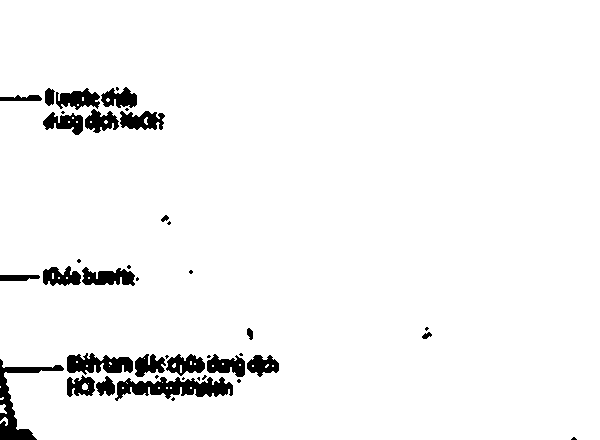
\includegraphics[width=6.0cm]{images_gk1_hoa11_ma1204/hinh_chuan_do_c5_hd.png}
\end{center}
Sau ba lần chuẩn độ, thể tích dung dịch $\ce{HCl}$ $0{,}1\,\text{M}$ đã dùng có giá trị trung bình là $15\,\text{mL}$. Giá trị của $x$ là
\choice
{\True 0,15 M}
{0,10 M}
{0,20 M}
{0,30 M}
\begin{loigiai}
Phương trình phản ứng chuẩn độ: $\ce{NaOH + HCl -> NaCl + H2O}$.\\
Tại điểm tương đương (chỉ thị đổi màu):
$$n_{\ce{NaOH}} = n_{\ce{HCl}} \Leftrightarrow C_{\ce{NaOH}} \cdot V_{\ce{NaOH}} = C_{\ce{HCl}} \cdot V_{\ce{HCl}}$$
$$\Leftrightarrow x \cdot 10 = 0{,}1 \cdot 15 \Rightarrow x = \dfrac{0{,}1 \cdot 15}{10} = 0{,}15\,\text{M}.$$
$\rightarrow$ \textbf{Chọn đáp án A.}
\end{loigiai}
\end{ex}


\begin{ex}%[1204-C6]
Ở trạng thái tự nhiên, nitrogen
\choice
{tự do chiếm khoảng 20\% thể tích không khí}
{\True tồn tại ở dạng đơn chất và hợp chất}
{chỉ tồn tại ở dạng đơn chất}
{chỉ tồn tại ở dạng hợp chất}
\begin{loigiai}
Ở trạng thái tự nhiên, nitrogen tồn tại ở cả dạng đơn chất (khí $\ce{N2}$ chiếm khoảng 78\% thể tích không khí) và dạng hợp chất (trong khoáng vật diêm tiêu $\ce{NaNO3}$, protein, nucleic acid trong tế bào sinh vật,...).\\
$\rightarrow$ \textbf{Chọn đáp án B.}
\end{loigiai}
\end{ex}


\begin{ex}%[1204-C7]
Các gói bim bim được làm phồng lên bằng khí X không màu, không mùi, trơ về mặt hóa học giúp tăng thời gian bảo quản và giữ được hình dạng sản phẩm không bị vỡ vụn. X là khí nào sau đây?
\choice
{\ce{NH3}}
{\ce{O2}}
{\True \ce{N2}}
{\ce{O3}}
\begin{loigiai}
Khí nitrogen ($\ce{N2}$) có liên kết ba $\ce{N#N}$ bền vững với năng lượng liên kết lớn ($945\,\text{kJ/mol}$) nên trơ về mặt hóa học ở nhiệt độ thường. Khí $\ce{N2}$ không màu, không mùi, không độc, được bơm vào bao bì bim bim/snack để bảo vệ thực phẩm chống oxi hóa và giữ khuôn sản phẩm không bị vỡ vụn khi va chạm.\\
$\rightarrow$ \textbf{Chọn đáp án C.}
\end{loigiai}
\end{ex}


\begin{ex}%[1204-C8]
Phản ứng nào sau đây là phản ứng thuận nghịch?
\choice
{\True $\ce{N2 + O2 <=>[t^\circ] 2NO}$}
{$\ce{C2H5OH + 3O2 ->[t^\circ] 2CO2 + 3H2O}$}
{$\ce{2KClO3 ->[t^\circ] 2KCl + 3O2}$}
{$\ce{Mg + 2HCl -> MgCl2 + H2}$}
\begin{loigiai}
Ở nhiệt độ cao khoảng $3000^\circ\text{C}$ hoặc có tia lửa điện, $\ce{N2}$ tác dụng thuận nghịch với $\ce{O2}$ tạo ra $\ce{NO}$: $\ce{N2(g) + O2(g) <=> 2NO(g)}$. Các phản ứng còn lại đều diễn ra một chiều.\\
$\rightarrow$ \textbf{Chọn đáp án A.}
\end{loigiai}
\end{ex}


\begin{ex}%[1204-C9]
Hòa tan một ít tinh thể $\ce{CH3COONa}$ vào ống nghiệm chứa nước, có tồn tại cân bằng sau:
$$\ce{CH3COONa + H2O <=> CH3COOH + NaOH}\quad (1)$$
Thêm vài giọt phenolphthalein vào ống nghiệm thấy dung dịch chuyển sang màu hồng nhạt, tiến hành ngâm ống nghiệm trong nước nóng màu dung dịch đậm dần. Kết luận nào sau đây chính xác?
\choice
{Khi tăng nhiệt độ, cân bằng (1) chuyển dịch theo chiều nghịch}
{\True Nếu ngâm ống nghiệm trong nước đá, màu dung dịch nhạt dần}
{Chiều thuận của phản ứng (1) là quá trình tỏa nhiệt}
{Cân bằng (1) không phụ thuộc vào nhiệt độ}
\begin{loigiai}
Cân bằng thủy phân: $\ce{CH3COO- + H2O <=> CH3COOH + OH-}$.\\
Màu hồng nhạt do ion $\ce{OH-}$ tạo ra. Khi ngâm vào nước nóng (tăng nhiệt độ), màu dung dịch đậm dần $\Rightarrow$ nồng độ $\ce{OH-}$ tăng $\Rightarrow$ cân bằng chuyển dịch theo chiều thuận. Theo nguyên lí Le Chatelier, khi tăng nhiệt độ cân bằng chuyển dịch theo chiều thu nhiệt $\Rightarrow$ chiều thuận là quá trình thu nhiệt ($\Delta H > 0$).\\
Do đó, khi ngâm vào nước đá (hạ nhiệt độ), cân bằng sẽ chuyển dịch theo chiều tỏa nhiệt (chiều nghịch), làm giảm nồng độ $\ce{OH-}$ nên màu dung dịch nhạt dần.\\
$\rightarrow$ \textbf{Chọn đáp án B.}
\end{loigiai}
\end{ex}


\begin{ex}%[1204-C10]
Phân tử ammonia được tạo thành bởi một nguyên tử nitrogen liên kết với ba nguyên tử hydrogen. Dạng hình học của phân tử ammonia là
\choice
{\True chóp tam giác}
{tứ giác}
{tam giác đều}
{vuông phẳng}
\begin{loigiai}
Nguyên tử nitrogen trong phân tử $\ce{NH3}$ ở trạng thái lai hóa $\text{sp}^3$, tạo 3 liên kết $\sigma$ với 3 nguyên tử hydrogen và còn 1 cặp electron tự do không liên kết. Cặp electron này chiếm không gian đẩy các liên kết $\ce{N-H}$ cụp xuống tạo nên cấu trúc hình chóp tam giác (tháp tam giác) với góc liên kết $\widehat{\text{HNH}} \approx 107^\circ$.\\
$\rightarrow$ \textbf{Chọn đáp án A.}
\end{loigiai}
\end{ex}


\begin{ex}%[1204-C11]
Chất nào sau đây khi hòa tan vào nước không phân li ra ion ?
\choice
{\ce{CH3COOH}}
{\True \ce{C2H5OH}}
{\ce{HCl}}
{\ce{NaCl}}
\begin{loigiai}
$\ce{C2H5OH}$ (ethanol) là chất không điện li, khi tan vào nước chỉ phân tán thành các phân tử $\ce{C2H5OH}$ ngậm nước, không phân li ra các ion. $\ce{CH3COOH}$ là chất điện li yếu; $\ce{HCl}$ và $\ce{NaCl}$ là các chất điện li mạnh.\\
$\rightarrow$ \textbf{Chọn đáp án B.}
\end{loigiai}
\end{ex}


\begin{ex}%[1204-C12]
Trong quá trình đốt cháy nhiên liệu hóa thạch như than đá và dầu nặng, thường sản sinh các khí $\ce{NO, NO2}\dots$ Tên gọi của $\ce{NO2}$ là
\choice
{ammonia}
{\True nitrogen dioxide}
{dinitrogen oxide}
{nitrogen monoxide}
\begin{loigiai}
$\ce{NO2}$ có tên gọi theo danh pháp quốc tế là nitrogen dioxide ($\ce{NO}$ là nitrogen monoxide; $\ce{N2O}$ là dinitrogen oxide; $\ce{NH3}$ là ammonia).\\
$\rightarrow$ \textbf{Chọn đáp án B.}
\end{loigiai}
\end{ex}


\vspace{6pt}
\noindent
\textbf{\large\color{mainGreen}PHẦN II. Câu trắc nghiệm đúng sai (2,0 điểm)}

\textit{Học sinh trả lời từ câu 1 đến câu 2. Trong mỗi ý a), b), c), d) ở mỗi câu, học sinh chọn đúng hoặc sai.}
\vspace{4pt}


\begin{ex}%[1204-P2-C1]
Phương trình hóa học của phản ứng tổng hợp ammonia từ nitrogen và hydrogen bằng quá trình Haber như sau:
$$\ce{N2(g) + 3H2(g) <=>[t^\circ, p, \text{xt Fe}] 2NH3(g)}\quad \Delta_\text{r}H^\circ_{298} = -91{,}8\,\text{kJ}\quad (*)$$
\choiceTF
{\True Liên kết hoá học trong phân tử $\ce{NH3}$ là liên kết cộng hoá trị có cực}
{Do có hàm lượng nitrogen cao (82,35\% theo khối lượng) nên ammonia được sử dụng trực tiếp làm phân đạm rất hiệu quả}
{Có thể nhận biết muối ammonium bằng cách cho muối tác dụng với dung dịch kiềm thấy thoát ra chất khí làm quỳ tím ẩm hoá đỏ}
{\True Phản ứng (*) là phản ứng tỏa nhiệt. Để tăng hiệu suất tổng hợp $\ce{NH3}$ người ta cần thực hiện ở nhiệt độ thấp nhưng không quá thấp để tốc độ phản ứng không quá chậm}
\begin{loigiai}
\begin{itemize}[leftmargin=1.5cm]
\item[\textbf{a) ĐÚNG:}] Do độ âm điện của $\ce{N}$ ($3{,}04$) lớn hơn $\ce{H}$ ($2{,}20$) nên 3 liên kết $\ce{N-H}$ đều là liên kết cộng hóa trị có cực, cặp electron dùng chung lệch về phía nguyên tử nitrogen.
\item[\textbf{b) SAI:}] Ammonia ở điều kiện thường là chất khí có tính ăn mòn, mùi khai xốc độc hại và bay hơi nhanh gây thất thoát N, nên $\ce{NH3}$ không được dùng trực tiếp làm phân đạm mà dùng làm nguyên liệu tổng hợp các loại phân đạm rắn như urea, đạm ammonium.
\item[\textbf{c) SAI:}] Khí thoát ra là $\ce{NH3}$ có tính base: $\ce{NH4+ + OH- -> NH3 ^ + H2O}$. Khí $\ce{NH3}$ làm quỳ tím ẩm \textbf{hóa xanh} (chứ không phải hóa đỏ).
\item[\textbf{d) ĐÚNG:}] Phản ứng có $\Delta_\text{r}H^\circ_{298} = -91{,}8\,\text{kJ} < 0$ nên là phản ứng tỏa nhiệt. Theo nguyên lí Le Chatelier, hạ nhiệt độ giúp cân bằng chuyển dịch theo chiều thuận. Tuy nhiên nếu hạ quá thấp tốc độ phản ứng sẽ rất chậm, do đó trong công nghiệp người ta chọn nhiệt độ tối ưu khoảng $400 - 450^\circ\text{C}$ cùng xúc tác $\ce{Fe}$.
\end{itemize}
\end{loigiai}
\end{ex}


\begin{ex}%[1204-P2-C2]
Ở các vùng quê, người dân thường dùng phèn chua ($\ce{K2SO4.Al2(SO4)3.24H2O}$ hay $\ce{KAl(SO4)2.12H2O}$) để làm trong nước. Khi phèn chua tan vào nước thì ion $\ce{Al^{3+}}$ bị thủy phân theo phản ứng:
$$\ce{Al^{3+} + 3H2O <=> Al(OH)3 + 3H+}\quad (*)$$
\choiceTF
{\True Phèn chua là chất điện li}
{\True Dung dịch sau khi hoà tan phèn chua vào nước có $\text{pH} < 7$}
{Dung dịch phèn chua làm phenolphthalein chuyển sang màu hồng}
{Phèn chua được dùng để làm trong nước nhờ ứng dụng của phản ứng thuỷ phân ion $\ce{Al^{3+}}$. Các bụi bẩn sẽ bị cuốn theo kết tủa keo trắng $\ce{Al(OH)3}$ lắng xuống đáy nên nước sẽ trong lại. Trong phản ứng (*) $\ce{Al^{3+}}$ là base và $\ce{H2O}$ là acid}
\begin{loigiai}
\begin{itemize}[leftmargin=1.5cm]
\item[\textbf{a) ĐÚNG:}] Phèn chua là muối kép của kim loại, khi hòa tan vào nước phân li hoàn toàn thành các ion $\ce{K+, Al^{3+}, SO4^{2-}}$ nên là chất điện li mạnh.
\item[\textbf{b) ĐÚNG:}] Do quá trình thủy phân của ion $\ce{Al^{3+}}$ tạo ra môi trường chứa ion $\ce{H+}$, nồng độ $[\ce{H+}] > 10^{-7}\,\text{M}$ nên dung dịch có tính acid, $\text{pH} < 7$.
\item[\textbf{c) SAI:}] Phenolphthalein chỉ chuyển sang màu hồng trong môi trường base ($\text{pH} > 8{,}3$). Dung dịch phèn chua có tính acid nên phenolphthalein không chuyển màu (vẫn không màu).
\item[\textbf{d) SAI:}] Phần đầu phát biểu đúng về ứng dụng tạo kết tủa keo $\ce{Al(OH)3}$ kéo theo chất bẩn lắng xuống. Tuy nhiên trong phản ứng (*), theo thuyết Brønsted -- Lowry, ion $\ce{Al^{3+}}$ (trong phức aqua $\ce{[Al(H2O)6]^{3+}}$) nhường proton $\ce{H+}$ nên đóng vai trò là \textbf{acid}, còn $\ce{H2O}$ nhận proton $\ce{H+}$ nên đóng vai trò là \textbf{base}.
\end{itemize}
\end{loigiai}
\end{ex}


\vspace{6pt}
\noindent
\textbf{\large\color{mainGreen}PHẦN III. Câu trắc nghiệm trả lời ngắn (2,0 điểm)}

\textit{Học sinh trả lời từ câu 1 đến câu 4.}
\vspace{4pt}


\begin{ex}%[1204-P3-C1]
Trong thí nghiệm chuẩn độ dung dịch $\ce{NaOH}$ bằng dung dịch $\ce{HCl}$, người ta cho từ từ dung dịch $\ce{NaOH}$ từ burette vào bình tam giác chứa dung dịch $\ce{HCl}$ và vài giọt dung dịch phenolphthalein. Trong các dụng cụ thí nghiệm được đánh số dưới đây, burette là dụng cụ số mấy?
\begin{center}
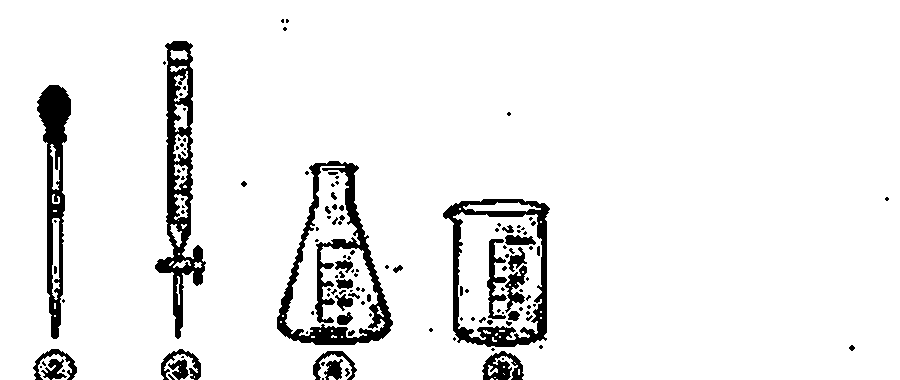
\includegraphics[width=11.5cm]{images_gk1_hoa11_ma1204/dung_cu_thi_nghiem_hd.png}
\end{center}
\textbf{Trả lời: } \textbf{\color{hfRed}3}
\begin{loigiai}
Nhận dạng các dụng cụ thí nghiệm trên hình vẽ:\\
(1) Ống đong (Measuring cylinder).\\
(2) Ống hút nhỏ giọt / pipet (Dropper pipette).\\
(3) \textbf{Burette} (buret kẹp trên giá sắt dùng để chuẩn độ dung dịch).\\
(4) Bình tam giác / bình nón (Erlenmeyer flask).\\
(5) Cốc thủy tinh (Beaker).\\
Vậy burette là dụng cụ số \textbf{3}.
\end{loigiai}
\end{ex}


\begin{ex}%[1204-P3-C2]
Cho các ứng dụng sau:
\begin{enumerate}[label=(\arabic*)]
\item Sản xuất phân đạm urea ($\ce{(NH2)2CO}$).
\item Được sử dụng làm chất làm lạnh trong thiết bị lạnh.
\item Sản xuất nitrogen.
\item Sản xuất nitric acid.
\end{enumerate}
Hãy liệt kê các ứng dụng đúng của ammonia theo thứ tự tăng dần? (Ví dụ: 123, 234...)

\textbf{Trả lời: } \textbf{\color{hfRed}124}
\begin{loigiai}
Phân tích các ứng dụng của ammonia ($\ce{NH3}$):\\
(1) ĐÚNG: Sản xuất phân đạm urea: $\ce{2NH3 + CO2 -> (NH2)2CO + H2O}$.\\
(2) ĐÚNG: Dễ hóa lỏng, nhiệt hóa hơi lớn nên dùng làm chất sinh hàn trong thiết bị lạnh công nghiệp.\\
(3) SAI: Trong công nghiệp, $\ce{N2}$ được sản xuất từ không khí lỏng, không ai dùng $\ce{NH3}$ để sản xuất $\ce{N2}$.\\
(4) ĐÚNG: Sản xuất nitric acid qua quá trình Ostwald ($\ce{NH3 -> NO -> NO2 -> HNO3}$).\\
Các ứng dụng đúng là (1), (2), (4). Viết theo thứ tự tăng dần là \textbf{124}.
\end{loigiai}
\end{ex}


\begin{ex}%[1204-P3-C3]
Cho phản ứng thuận nghịch sau ở nhiệt độ $430^\circ\text{C}$: $\ce{H2(g) + I2(g) <=> 2HI(g)}$. Nồng độ mol các chất ở thời điểm cân bằng như sau: $[\ce{H2}] = [\ce{I2}] = 0{,}107\,\text{M}$; $[\ce{HI}] = 0{,}768\,\text{M}$. Tính hằng số cân bằng $K_\text{c}$ của phản ứng ở $430^\circ\text{C}$ (làm tròn kết quả đến hàng phần mười).

\textbf{Trả lời: } \textbf{\color{hfRed}51,5}
\begin{loigiai}
Biểu thức hằng số cân bằng của phản ứng:\\
$$K_\text{c} = \dfrac{[\ce{HI}]^2}{[\ce{H2}]\cdot[\ce{I2}]} = \dfrac{(0{,}768)^2}{0{,}107 \cdot 0{,}107} = \dfrac{0{,}589824}{0{,}011449} \approx 51{,}5175\dots$$
Làm tròn kết quả đến hàng phần mười: $K_\text{c} = \mathbf{51{,}5}$.
\end{loigiai}
\end{ex}


\begin{ex}%[1204-P3-C4]
Cho các phát biểu sau:
\begin{enumerate}[label=(\arabic*)]
\item Ánh sáng mặt trời bị cản trở làm ảnh hưởng đến quá trình quang hợp, gây thiếu oxygen làm cho thực vật và động vật chết.
\item Sự phân hủy xác động thực vật bởi vi khuẩn sử dụng nhiều oxygen trong nước gây nên tình trạng thiếu oxygen nghiêm trọng, làm chết cả hệ sinh thái.
\item Chất dinh dưỡng giúp thực vật và tảo sống trong nước phát triển ồ ạt.
\item Phân bón và chất dinh dưỡng bị rửa trôi xuống sông, ao, hồ.
\end{enumerate}
Hãy sắp xếp các phát biểu trên theo đúng trình tự diễn biến quá trình hình thành hiện tượng phú dưỡng thành bộ bốn số (ví dụ: 2143, 4213, ...)?

\textbf{Trả lời: } \textbf{\color{hfRed}4312}
\begin{loigiai}
Trình tự diễn biến quá trình phú dưỡng (Eutrophication):\\
(4) Nguồn phân bón dư thừa và chất dinh dưỡng bị nước mưa rửa trôi xuống sông, ao, hồ.\\
$\rightarrow$ (3) Chất dinh dưỡng kích thích thực vật thủy sinh và tảo sống trong nước phát triển bùng phát, ồ ạt.\\
$\rightarrow$ (1) Thảm thực vật/tảo dày đặc che lấp ánh sáng mặt trời, cản trở quá trình quang hợp và gây thiếu oxygen khiến sinh vật bắt đầu chết.\\
$\rightarrow$ (2) Quá trình phân hủy xác động thực vật bởi vi khuẩn tiêu tốn nhiều oxygen trong nước gây thiếu hụt oxygen nghiêm trọng, hủy hoại cả hệ sinh thái.\\
Trình tự diễn biến đúng là: (4) $\rightarrow$ (3) $\rightarrow$ (1) $\rightarrow$ (2). Bộ bốn số là \textbf{4312}.
\end{loigiai}
\end{ex}


\vspace{6pt}
\noindent
\textbf{\large\color{hfRed}B. PHẦN TỰ LUẬN (3,0 ĐIỂM)}
\vspace{4pt}


\begin{ex}%[1204-TL1]
\textbf{(1,0 điểm)} Cho cân bằng hoá học (trong bình kín) sau:
$$\ce{2NO2 (g) <=> N2O4 (g)}\quad (*)$$
\quad\quad\quad\quad\textit{(màu nâu đỏ)}\quad\quad\quad\textit{(không màu)}
\begin{enumerate}[label=\textbf{\alph*)}]
\item Cân bằng (*) chuyển dịch theo chiều nào (thuận hay nghịch) khi tăng áp suất của hỗn hợp ở điều kiện nhiệt độ không đổi? Giải thích ngắn gọn.
\item Khi hạ nhiệt độ của bình thì màu nâu đỏ nhạt dần. Phản ứng thuận là toả nhiệt hay thu nhiệt? (không giải thích).
\end{enumerate}
\begin{loigiai}
\textbf{a) (0,5 điểm)}
\begin{itemize}[leftmargin=0.8cm]
\item Khi tăng áp suất của hệ phản ứng ở nhiệt độ không đổi, theo nguyên lí Le Chatelier, cân bằng sẽ chuyển dịch theo chiều làm giảm áp suất của hệ, tức là chiều làm giảm tổng số mol khí.
\item Xét phản ứng (*): vế trái có $2\,\text{mol}$ khí ($\ce{NO2}$), vế phải có $1\,\text{mol}$ khí ($\ce{N2O4}$). Số mol khí giảm theo chiều từ trái sang phải.
\item Do đó, cân bằng (*) chuyển dịch theo \textbf{CHIỀU THUẬN}.
\end{itemize}
\textbf{b) (0,5 điểm)}
\begin{itemize}[leftmargin=0.8cm]
\item Khi hạ nhiệt độ, màu nâu đỏ nhạt dần chứng tỏ nồng độ $\ce{NO2}$ giảm và nồng độ $\ce{N2O4}$ tăng lên $\Rightarrow$ Cân bằng chuyển dịch theo chiều thuận.
\item Theo nguyên lí Le Chatelier, khi hạ nhiệt độ cân bằng chuyển dịch theo chiều tỏa nhiệt để chống lại sự giảm nhiệt độ.
\item Vậy phản ứng thuận là phản ứng \textbf{TỎA NHIỆT}.
\end{itemize}
\end{loigiai}
\end{ex}


\begin{ex}%[1204-TL2]
\textbf{(1,0 điểm)} Nước thải công nghiệp trước khi xả ra môi trường cần được thu gom và xử lý đạt tiêu chuẩn theo quy định. Theo quy chuẩn kỹ thuật quốc gia về nước thải công nghiệp, giá trị pH của nước thải công nghiệp khi xả vào nguồn tiếp nhận phải nằm trong khoảng từ 5,5 đến 9,0. Một mẫu nước thải của nhà máy X có $\text{pH} = 4$. Để đảm bảo đạt tiêu chuẩn xả thải, nhà máy sử dụng vôi sống ($\ce{CaO}$) cho vào nước thải để nâng pH từ 4 lên 7.
\begin{enumerate}[label=\textbf{\alph*)}]
\item Hãy cho biết mẫu nước thải của nhà máy X có môi trường là acid, base hay trung tính?
\item Giải thích tác dụng của vôi sống trong việc làm tăng pH của nước thải bằng phương trình hoá học?
\item Tính khối lượng vôi sống (kilogam) cần sử dụng để xử lý $6000\,\text{m}^3$ nước thải nói trên? (Bỏ qua sự thủy phân của các muối nếu có). (Không làm tròn kết quả các phép tính trung gian, chỉ làm tròn kết quả cuối cùng đến hàng phần mười).
\end{enumerate}
\begin{loigiai}
\textbf{a) (0,25 điểm)}
Mẫu nước thải có $\text{pH} = 4 < 7$ nên mẫu nước thải có \textbf{MÔI TRƯỜNG ACID}.\\

\textbf{b) (0,25 điểm)}
Khi cho vôi sống ($\ce{CaO}$) vào nước thải, xảy ra các phản ứng:
$$\ce{CaO + H2O -> Ca(OH)2}$$
$$\ce{Ca(OH)2 -> Ca^{2+} + 2OH-}$$
$$\ce{H+ + OH- -> H2O}\quad (\text{hoặc: }\ce{CaO + 2H+ -> Ca^{2+} + H2O})$$
Ion $\ce{OH-}$ sinh ra trung hòa bớt ion $\ce{H+}$ trong nước thải acid, làm giảm nồng độ $[\ce{H+}]$, do đó giá trị $\text{pH} = -\lg[\ce{H+}]$ của nước thải \textbf{tăng lên}.\\

\textbf{c) (0,5 điểm)}
\begin{itemize}[leftmargin=0.8cm]
\item Thể tích nước thải: $V = 6000\,\text{m}^3 = 6 \cdot 10^6\,\text{L}$.
\item Tại $\text{pH} = 4 \Rightarrow [\ce{H+}]_\text{đầu} = 10^{-4}\,\text{M}$.
\item Tại $\text{pH} = 7 \Rightarrow [\ce{H+}]_\text{sau} = 10^{-7}\,\text{M}$.
\item Lượng ion $\ce{H+}$ cần trung hòa là:
$$n_{\ce{H+}} = ([\ce{H+}]_\text{đầu} - [\ce{H+}]_\text{sau}) \cdot V = (10^{-4} - 10^{-7}) \cdot 6 \cdot 10^6 = 600 - 0{,}6 = 599{,}4\,\text{mol}.$$
\item Theo phản ứng: $\ce{CaO + 2H+ -> Ca^{2+} + H2O}$, ta có:
$$n_{\ce{CaO}} = \dfrac{1}{2} n_{\ce{H+}} = \dfrac{599{,}4}{2} = 299{,}7\,\text{mol}.$$
\item Khối lượng vôi sống ($M_{\ce{CaO}} = 40 + 16 = 56\,\text{g/mol}$) cần dùng:
$$m_{\ce{CaO}} = 299{,}7 \cdot 56 = 16783{,}2\,\text{g} = 16{,}7832\,\text{kg}.$$
\item Làm tròn kết quả đến hàng phần mười theo yêu cầu:
$$m_{\ce{CaO}} = \mathbf{16{,}8}\,\text{kg}.$$
\end{itemize}
\end{loigiai}
\end{ex}


\begin{ex}%[1204-TL3]
\textbf{(1,0 điểm)} Quá trình hình thành đạm nitrate cho đất từ nước mưa được biểu diễn theo sơ đồ sau:
$$\ce{N2 ==(1)==> NO ==(2)==> NO2 ==(3)==> HNO3 ==(4)==> H+ + NO3^-}$$
\begin{enumerate}[label=\textbf{\alph*)}]
\item Viết phương trình hóa học của các phản ứng xảy ra (ghi rõ điều kiện nếu có, mỗi mũi tên là một phản ứng hóa học).
\item Một cơn mưa rơi xuống một thửa ruộng với lượng mưa trung bình là $5\,\text{m}^3/\text{giờ}$. Hãy tính khối lượng nguyên tố nitrogen (tính bằng gam) mà thửa ruộng nhận được khi cơn mưa đó kéo dài 3 giờ? (Giả sử hàm lượng ion nitrate trong nước mưa khoảng $62\,\text{mg/L}$ và hàm lượng nitrate trong nước mưa không đổi trong suốt thời gian mưa).
\end{enumerate}
\begin{loigiai}
\textbf{a) (0,5 điểm)}
Các phương trình hóa học xảy ra theo sơ đồ:
\begin{align*}
(1)\quad &\ce{N2(g) + O2(g) <=>[3000^\circ\text{C}\text{ hoặc tia lửa điện}] 2NO(g)}\\
(2)\quad &\ce{2NO(g) + O2(g) -> 2NO2(g)}\\
(3)\quad &\ce{4NO2(g) + O2(g) + 2H2O(l) -> 4HNO3(aq)}\\
(4)\quad &\ce{HNO3(aq) -> H+(aq) + NO3^-(aq)}
\end{align*}
\textbf{b) (0,5 điểm)}
\begin{itemize}[leftmargin=0.8cm]
\item Thể tích nước mưa rơi xuống thửa ruộng trong 3 giờ:
$$V = 5\,\text{m}^3/\text{giờ} \cdot 3\,\text{giờ} = 15\,\text{m}^3 = 15\,000\,\text{L}.$$
\item Tổng khối lượng ion nitrate ($\ce{NO3-}$) có trong lượng nước mưa trên:
$$m_{\ce{NO3-}} = 62\,\text{mg/L} \cdot 15\,000\,\text{L} = 930\,000\,\text{mg} = 930\,\text{g}.$$
\item Khối lượng mol: $M_{\ce{NO3-}} = 62\,\text{g/mol}$; $M_{\ce{N}} = 14\,\text{g/mol}$.
\item Khối lượng nguyên tố nitrogen mà thửa ruộng nhận được (bảo toàn nguyên tố $\ce{N}$):
$$m_{\ce{N}} = m_{\ce{NO3-}} \cdot \dfrac{M_{\ce{N}}}{M_{\ce{NO3-}}} = 930 \cdot \dfrac{14}{62} = \mathbf{210}\,\text{g}.$$
\end{itemize}
\end{loigiai}
\end{ex}


\vspace{6pt}
\begin{center}
\textbf{---------- HẾT ----------}\\
\textit{\small - Thí sinh không được sử dụng tài liệu.\\
- Giám thị không giải thích gì thêm.}
\end{center}

\end{document}
